% Configure documentclass
\documentclass[a4paper,12pt,twoside]{article}

% Add common preamble to the document
%% This file is shared between thesis and proposal

\usepackage[scaled]{helvet}
\usepackage{url}
\usepackage{cite}
\usepackage{listings}
\usepackage[pdftex]{graphicx}
\usepackage[hang,small,bf]{caption}
\usepackage{styles/tum}
\usepackage{setspace}
\usepackage[german,english]{babel}
\usepackage{float}
\usepackage{floatflt}
\usepackage{fancyhdr}
\usepackage{color}
\usepackage{booktabs}
\usepackage[pdftex,bookmarks=true,plainpages=false,pdfpagelabels=true]{hyperref}	%TODO make yourself familiar with \label, \ref and \hyperref for referencing figures, tables, chapters, etc.
\usepackage{mdwlist}
\usepackage{enumerate}
\usepackage{array}
\usepackage{longtable}
\usepackage[utf8]{inputenc}
\usepackage[capitalize, noabbrev]{cleveref}
\usepackage{wasysym}
\usepackage{todonotes}

% Path for graphics
\graphicspath{{figures/}}

% Include the Thesis metadata like title, author, etc. 
\input{metadata}

%%%%%%%%%%%%%%%%%%%%%%%%%%%%%%%%%%%%%%%%%%%%%%%%%%%%%%%%%%%%%%%%%%%%%%%%%%%%%%%%%%%%%%%%%%%%%%%%%
% Custom Commands for this template
%%%%%%%%%%%%%%%%%%%%%%%%%%%%%%%%%%%%%%%%%%%%%%%%%%%%%%%%%%%%%%%%%%%%%%%%%%%%%%%%%%%%%%%%%%%%%%%%%

% Annotate feedback you received 
\newcommand{\feedback}[1]{\todo[inline,color=green,caption={}]{#1}}

% State what is missing in this spot
\newcommand{\missing}[1]{\todo[inline,color=yellow,caption={}]{#1}}

% Inline to do note: 
\newcommand{\TODO}[1]{\todo[inline,caption={}]{#1}}





\def\proposal{Proposal for}

%%%%%%%%%%%%%%%%%%%%%%%%%%%%%%%%%%%%%%%%%%%%%%%%%%%%%%%%%%%
% Theses specific packages go here
%%%%%%%%%%%%%%%%%%%%%%%%%%%%%%%%%%%%%%%%%%%%%%%%%%%%%%%%%%%
\usepackage[nolist]{acronym}
\begin{acronym}
        \acro{AL}{Adaptive Learning}
        \acro{CIT}{School of Computation, Information and Technology}
        \acro{LMS}{Learning Management System}
        \acro{SRL}{self-Regulated Learning}
        \acro{TUM}{Technical University of Munich}
\end{acronym}

%%%%%%%%%%%%%%%%%%%%%%%%%%%%%%%%%%%%%%%%%%%%%%%%%%%%%%%%%%%
% Begin of document
%%%%%%%%%%%%%%%%%%%%%%%%%%%%%%%%%%%%%%%%%%%%%%%%%%%%%%%%%%%
\begin{document}
\setlength{\evensidemargin}{22pt}
\setlength{\oddsidemargin}{22pt}


\hypersetup{pdfborder={0 0 0}, pdfauthor={\author}, pdftitle={\title}}

\lstset{showspaces=false, numbers=left, frame=single, basicstyle=\small}

%------- Title setup -------
\thispagestyle{empty}
{
\sffamily

\vspace{1cm}
\begin{center}
\oTUM{4cm}

\vspace{5mm}     
{\LARGE \bf \sffamily Technical University of Munich}

\vspace{5mm}
{\Large School of Computation, Information and Technology \\ -- Informatics -- }	
\vspace{1mm}
\end{center}

\vspace{15mm}

\begin{center}
        {\large {\proposal} {\degree}'s Thesis in \program}
\vspace{8mm}

\begin{spacing}{1.3}
{\LARGE \bf \sffamily \title}\\
\vspace{8mm}

{\LARGE \titleGer}\\
\vspace{8mm}
\end{spacing}

\begin{tabular}{ll}
\large Author:           & \large \author     \\[2mm]
\large Supervisor:       & \large \supervisor \\[2mm]				
\large Advisor:	         & \large \advisor    \\[2mm]
\ifx\proposal\empty\else
\large Start Date:       & \large \startdate  \\[2mm]
\fi
\large Submission Date:  & \large \date
\end{tabular}

\end{center}
}


\selectlanguage{english}
\pagenumbering{arabic}

\fancyhead{}
\pagestyle{fancy}
\fancyhead[LE]{\slshape \leftmark}
\fancyhead[RO]{\slshape \rightmark}
\headheight=15pt

%------- Start of Proposal -------
%\TODO{Before you start with your thesis, have a look at our guides on confluence! \url{https://confluence.ase.in.tum.de/display/EduResStud/How+to+thesis}}
\section{Introduction}
%\missing{ Introduction
%        \begin{itemize}
%                \item Introduce the reader to the general setting
%                \item What is the environment?
%                \item What are the tools in use?
%        \end{itemize}
%}

The wide availability of technology has changed the way students learn as well as the design of learning environments by instructors. Numerous
institutions have already integrated online learning into their teaching and are exploring new possibilities. \textit{Artemis}
\footnote{https://github.com/ls1intum/Artemis} is an \ac{LMS} developed at und used by the \ac{CIT} at \ac{TUM} and other universities.
By allowing instructors to create interactive exercises, automation of feedback as well as grading, the educational tool aims to reduce the
workload of instructors whilst maintaining a high-quality learning experience for students. Fuchs and Waldhauser have already added support
for learning and teaching analytics \cite{fuchs2021,waldhauser2021}. Aberle contributions extended the possibilities to assign exercises to competencies and create relations
between such, effectively setting the foundation for the integration of \ac{AL} in Artemis \cite{aberle2022}.

% more students, more online, new possibilites
% first steps towards adaptive learning
% competency relations

\section{Problem}
%\missing{ Problem description
%        \begin{itemize}
%                \item What is/are the problem(s)?
%                \item Identify the actors and use these to describe how the problem negatively influences them.
%                \item Do not present solutions or alternatives yet!
%                \item Present the negative consequences in detail
%        \end{itemize}
%}

Large-scale courses with up to 2000 users make it increasingly difficult for instructors to account for students' individual needs. In such large groups,
instructors inevitably encounter students with vastly different backgrounds, abilities, ages, and experiences \cite{mulryan2010teaching}. Currently, Artemis
incorporates little to no features that support instructors' efforts to provide students with individualized material. This lack of individualization
may cause students to be either bored or overwhelmed, situations that might impact the learning outcome and even mental-health \cite{graciani2020m, kadison2004college}.

Finally, the addition of dashboards for self-evaluation has improved the situation in regard of \ac{SRL}, however, the platform does not actively promote
\ac{SRL}.


\section{Motivation}
%\missing{ Thesis Motivation
%        \begin{itemize}
%                \item Outline why it is important to solve the problem
%                \item Again use the actors to present your solution, but don't be to specific
%                \item Be visionary!
%                \item If applicable, motivate with existing research, previous work
%        \end{itemize}
%}

On-demand availability of learning material on Artemis has given students a great degree of freedom to plan their learning experiences. Nonetheless, research
indicates that students may require assistance to do so effectively \cite{latham1991self}. Moreover, Artemis already collects a variety of data that can be used to analyze
the capabilities of individual students. Therefore, this information can be used to provide an adaptive learning experience. Research has shown that
\ac{AL} can improve learning outcomes significantly \cite{liu2017investigating}.

Furthermore, the implementation of \ac{AL} may incorporate features to allow for and promote \ac{SRL}. According to TEAL
"good self-regulators have developed the skills and habits to be effective learners, exhibit effective learning strategies, effort, and persistence" \cite{no2012self}.
Characteristics that instructors certainly want to foster in their students.

% reduce extraneous load
% self regulated learning
% adaptive learning

\section{Objective}
%\missing{ Thesis Objective
%        \begin{itemize}
%                \item What are the main goals of your thesis?
%        \end{itemize}
%}

This thesis will focus on the integration of \ac{AL} into Artemis.
Theoretical research and a requirements analysis will be used to create a software design based on the existing architecture of Artemis. The proposed
design will be implemented in the \ac{LMS}. Finally, the thesis will document the analysis of the current state, the requirements engineering process,
and the development of the features proposed in this section.

The following figures depict the proposed use cases and the analysis object model. The features are explained in detail in the consecutive subsections.

\begin{figure}[h!]
        \centering
        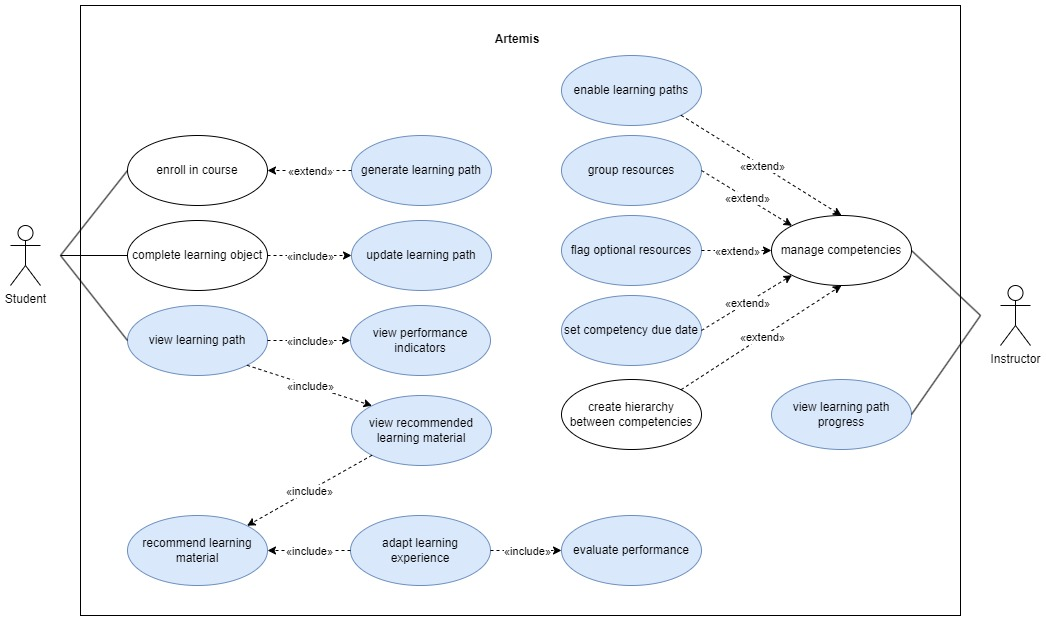
\includegraphics[width=\linewidth]{figures/UseCases(3).jpg}
        \caption{Use Cases related to adaptive learning in Artemis (new use cases are highlighted).}
        \label{fig:UseCases}
\end{figure}

\begin{figure}[h!]
        \centering
        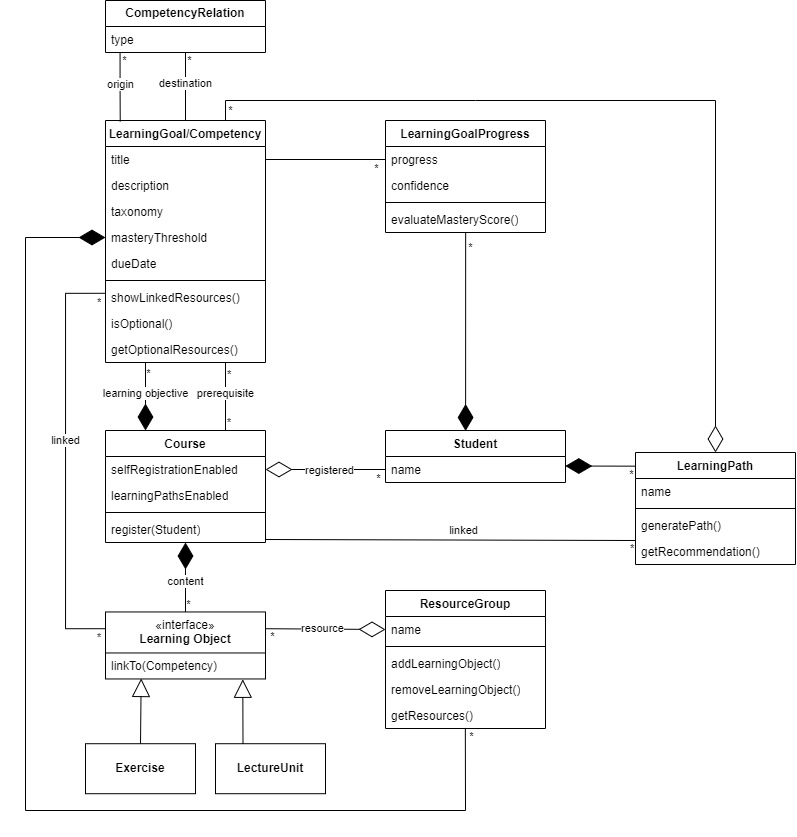
\includegraphics[width=\linewidth]{figures/ObjectModel (3).jpg}
        \caption{Analysis Object Model for the proposed features and use cases (additions are highlighted).}
        \label{fig:AOM}
\end{figure}

\subsection{Competency Management Improvements}
To allow for individual learning paths, instructors must be able to configure competencies in more detail. Firstly, instructors should be
able to bundle exercises that represent a variety of different difficulty levels, s.t. the learning path generation can later on cater exercises
with an appropriate complexity to the individual students.

Furthermore, instructors should be able to flag competencies or specific exercises as optional material. Therefore, ambitious students' learning paths
may incorporate these tasks to maintain the relatively high level of difficulty that these students may expect to keep them motivated.
On the other hand, the learning path system can omit these exercises for students that fall behind and provide alternative resources to allow them
to reiterate and gain more confidence with the required learning material.
It should be noted, that both of the before-mentioned features should exclude exercises that contribute towards the course score.

Finally, instructors should be able to configure deadlines for individual competencies. Therefore, students can get feedback if they are on track with the
expected progress.

\subsection{Learning Path Generation}
Once a student enrolls in a course, the system should create an individual learning path. The learning path should keep track of the student's progress and evaluate
their skill level based on several indicators, e.g. completion, score, elapsed time, and number of submissions. Based on this evaluation the system should
recommend suitable lecture units or exercises to fit the individual's needs.

\subsection{Student View}
Students must be able to view their progress in their learning path. There should be an intuitive representation of the already completed and upcoming tasks.
Furthermore, students should be able to review whether their progression is within the instructor's expectations regarding time. Further feedback indicators
representing the student's performance compared to other enrolled students might be beneficial to promote self-regulatory learning.
The overview should also incorporate the recommendation made by the learning path generation. Hence, students spend less time choosing their next task and can fluently
continue throughout their learning experience.

\subsection{Learning Analytics}
The application must incorporate a dashboard for instructors to analyze the progress of the participating students. To review the effectiveness of the learning material,
instructors need access to indicators, such as average completion of competencies, average participation in exercises, and average score of exercises.
Furthermore, instructors should be able to get insight into individual students' learning paths to allow for individual feedback.


\section{Schedule}
%\missing{ Thesis Schedule
%        \begin{itemize}
%                \item When will the thesis Start (Always 15th of Month)
%                \item Create a rough plan for your thesis (separate the time in sprints with a length of 2-4 Weeks)
%                \item Each sprint should contain several work items - Again keep it high-level and make to keep your plan realistic
%                \item Make sure the work-items are measurable and deliverable
%                \item No writing related tasks! (e.g. "Write Analysis Chapter")
%        \end{itemize}
%}

\begin{itemize}
        \item \textbf{Sprint I} End of May (Week 20-21): Improve Competency Managment
              \begin{itemize}
                      \item Instructors can remove competencies
                      \item Instructors can select due-dates for competencies
              \end{itemize}

        \item \textbf{Sprint II} Mid of June (Week 22-23): Improve Competency Managment
              \begin{itemize}
                      \item Instructors can set competencies as optional
                      \item Instructors can set specific exercises or lecture units as optional
              \end{itemize}

        \item \textbf{Sprint III} End of June (Week 24-25): Improve Competency Management
              \begin{itemize}
                      \item Instructors can generate exercise groups that represent a variety of different difficulty levels
              \end{itemize}

        \item \textbf{Sprint IV} Beginning of July (Week 26-27): Learning Path Generation
              \begin{itemize}
                      \item Instrucors can enable Learning Paths
                      \item Artemis generates a Learning Path for each Student
              \end{itemize}

        \item \textbf{Sprint V} Beginning of August (Week 28-29): Student \& Instructor View
              \begin{itemize}
                      \item Students can view their Learning Path
                      \item Instructors can view students' Learning Paths
              \end{itemize}

        \item \textbf{Sprint VI} Mid of August (Week 30-31): Learning Path Generation
              \begin{itemize}
                      \item Artemis evaluates students' performance
                      \item Artemis calculates recommendations for learning material based on students' performance
              \end{itemize}

        \item \textbf{Sprint VII} Beginning of September (Week 32-34): Learning Path Generation
              \begin{itemize}
                      \item Students can view recommended material in their Learning Path
                      \item Students can view performance indicators in their Learning Path
              \end{itemize}
\end{itemize}

\clearpage
\begin{acronym}
    \acro{GUI}{Graphical User Interface}

    \acro{AL}{Adaptive Learning}
    \acro{CIT}{School of Computation, Information and Technology}
    \acro{LMS}{Learning Management System}
    \acro{SRL}{self-Regulated Learning}
    \acro{TUM}{Technical University of Munich}
\end{acronym}

\clearpage
\bibliography{thesis}
\bibliographystyle{alpha}

\end{document}
